% !TEX root = main.tex
\section{Longitudinal relaxation measurements T1}
\label{sec:LongitudinalrelaxationmeasurementsT1}
There exist two possibilities to measure the longitudinal spin lattice relaxation.
First we want to have a closer look at the measurement via $\tau_p$ (polarizing pulse duration).
Therefore the computer program \textit{Prospa} applies a polarizing pulse orthogonal to the earths magnetic field.
Due to this polarizing pulse the spins align in the transversal plain and form a bulk magnetization.
By time the magnetization becomes stronger because of this the signal becomes stronger.
This relation is visualized in the figure \ref{fig:BildT1}.

\begin{figure}[H]
    \centering
    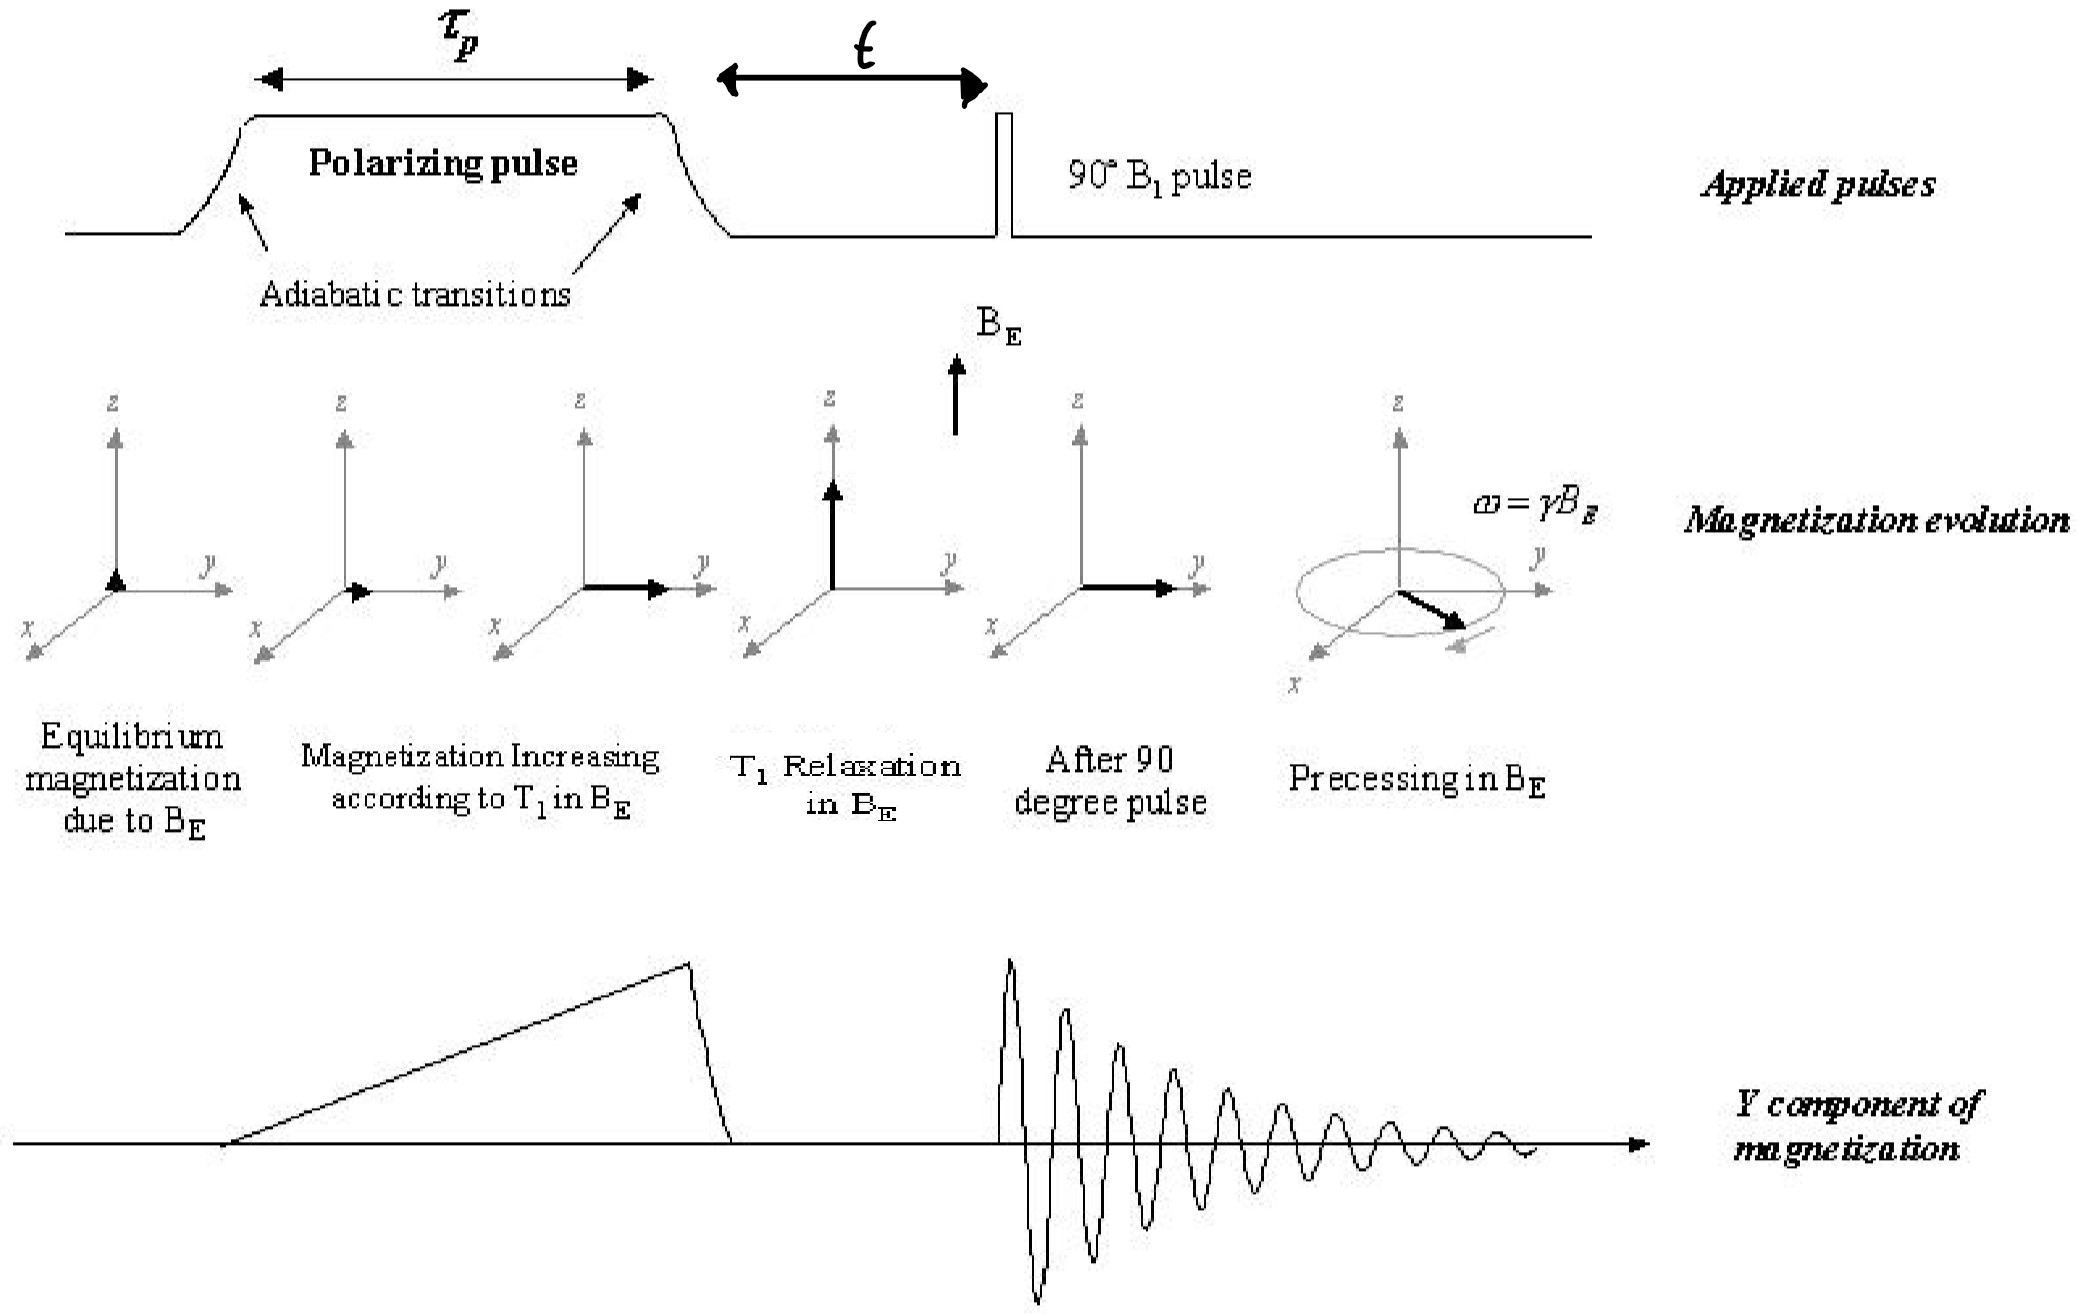
\includegraphics[width= \textwidth]{Abbildungen/BildT1.png}   
    \caption[Sketch to show how T$_1$ can be measured. \cite{Bild}]{Sketch to show how T$_1$ can be measured.
    One way is by changing the polarizing pulse duration $\tau_p$ and the other way is by varying the time between the polarizing pulse and the \SI{90}{\degree} pulse. \cite{Bild}}
    \label{fig:BildT1}
\end{figure}

Due to the increasing magnetization it is possible to calculate the T$_{1,p}$ relaxation.
In order to do so the magnetization time is increased step by step from \SI{500}{\milli \second} to \SI{4500}{\milli \second} with an increment of \SI{500}{\milli \second} and in each configuration the signals maximum is obtained from the fourier transformed spectrum.
Figure \ref{fig:T1Polarisationsfeldfeld} shows the attenuation of the signals normalized to the maximum peak E$_0$.
The underlying idea is that by applying a fit function as following:
\begin{align}
    S(x)=S_0 \cdot \left[1-\exp\left(\frac{-x}{T_{1,p}}\right)\right] \ ,
    \label{eq: fitBp}
\end{align}
it is possible to calculate the relaxation time T$_{1,p}$.
The exponential decay is a result of the loss of phase coherence between the spins and will be used for every measurement of spin relaxation.
In this case T$_{1,p}$ is found to count as \SI{2912.8800 \pm 0.0048}{\milli \second}.

\begin{figure}[H]
    \centering
    % GNUPLOT: LaTeX picture with Postscript
\begingroup
  % Encoding inside the plot.  In the header of your document, this encoding
  % should to defined, e.g., by using
  % \usepackage[cp1252,<other encodings>]{inputenc}
  \inputencoding{cp1252}%
  \makeatletter
  \providecommand\color[2][]{%
    \GenericError{(gnuplot) \space\space\space\@spaces}{%
      Package color not loaded in conjunction with
      terminal option `colourtext'%
    }{See the gnuplot documentation for explanation.%
    }{Either use 'blacktext' in gnuplot or load the package
      color.sty in LaTeX.}%
    \renewcommand\color[2][]{}%
  }%
  \providecommand\includegraphics[2][]{%
    \GenericError{(gnuplot) \space\space\space\@spaces}{%
      Package graphicx or graphics not loaded%
    }{See the gnuplot documentation for explanation.%
    }{The gnuplot epslatex terminal needs graphicx.sty or graphics.sty.}%
    \renewcommand\includegraphics[2][]{}%
  }%
  \providecommand\rotatebox[2]{#2}%
  \@ifundefined{ifGPcolor}{%
    \newif\ifGPcolor
    \GPcolorfalse
  }{}%
  \@ifundefined{ifGPblacktext}{%
    \newif\ifGPblacktext
    \GPblacktexttrue
  }{}%
  % define a \g@addto@macro without @ in the name:
  \let\gplgaddtomacro\g@addto@macro
  % define empty templates for all commands taking text:
  \gdef\gplbacktext{}%
  \gdef\gplfronttext{}%
  \makeatother
  \ifGPblacktext
    % no textcolor at all
    \def\colorrgb#1{}%
    \def\colorgray#1{}%
  \else
    % gray or color?
    \ifGPcolor
      \def\colorrgb#1{\color[rgb]{#1}}%
      \def\colorgray#1{\color[gray]{#1}}%
      \expandafter\def\csname LTw\endcsname{\color{white}}%
      \expandafter\def\csname LTb\endcsname{\color{black}}%
      \expandafter\def\csname LTa\endcsname{\color{black}}%
      \expandafter\def\csname LT0\endcsname{\color[rgb]{1,0,0}}%
      \expandafter\def\csname LT1\endcsname{\color[rgb]{0,1,0}}%
      \expandafter\def\csname LT2\endcsname{\color[rgb]{0,0,1}}%
      \expandafter\def\csname LT3\endcsname{\color[rgb]{1,0,1}}%
      \expandafter\def\csname LT4\endcsname{\color[rgb]{0,1,1}}%
      \expandafter\def\csname LT5\endcsname{\color[rgb]{1,1,0}}%
      \expandafter\def\csname LT6\endcsname{\color[rgb]{0,0,0}}%
      \expandafter\def\csname LT7\endcsname{\color[rgb]{1,0.3,0}}%
      \expandafter\def\csname LT8\endcsname{\color[rgb]{0.5,0.5,0.5}}%
    \else
      % gray
      \def\colorrgb#1{\color{black}}%
      \def\colorgray#1{\color[gray]{#1}}%
      \expandafter\def\csname LTw\endcsname{\color{white}}%
      \expandafter\def\csname LTb\endcsname{\color{black}}%
      \expandafter\def\csname LTa\endcsname{\color{black}}%
      \expandafter\def\csname LT0\endcsname{\color{black}}%
      \expandafter\def\csname LT1\endcsname{\color{black}}%
      \expandafter\def\csname LT2\endcsname{\color{black}}%
      \expandafter\def\csname LT3\endcsname{\color{black}}%
      \expandafter\def\csname LT4\endcsname{\color{black}}%
      \expandafter\def\csname LT5\endcsname{\color{black}}%
      \expandafter\def\csname LT6\endcsname{\color{black}}%
      \expandafter\def\csname LT7\endcsname{\color{black}}%
      \expandafter\def\csname LT8\endcsname{\color{black}}%
    \fi
  \fi
    \setlength{\unitlength}{0.0500bp}%
    \ifx\gptboxheight\undefined%
      \newlength{\gptboxheight}%
      \newlength{\gptboxwidth}%
      \newsavebox{\gptboxtext}%
    \fi%
    \setlength{\fboxrule}{0.5pt}%
    \setlength{\fboxsep}{1pt}%
\begin{picture}(7200.00,5040.00)%
    \gplgaddtomacro\gplbacktext{%
      \csname LTb\endcsname%%
      \put(814,704){\makebox(0,0)[r]{\strut{}$0$}}%
      \put(814,1527){\makebox(0,0)[r]{\strut{}$0.2$}}%
      \put(814,2350){\makebox(0,0)[r]{\strut{}$0.4$}}%
      \put(814,3173){\makebox(0,0)[r]{\strut{}$0.6$}}%
      \put(814,3996){\makebox(0,0)[r]{\strut{}$0.8$}}%
      \put(814,4819){\makebox(0,0)[r]{\strut{}$1$}}%
      \put(946,484){\makebox(0,0){\strut{}$0$}}%
      \put(1660,484){\makebox(0,0){\strut{}$500$}}%
      \put(2375,484){\makebox(0,0){\strut{}$1000$}}%
      \put(3089,484){\makebox(0,0){\strut{}$1500$}}%
      \put(3803,484){\makebox(0,0){\strut{}$2000$}}%
      \put(4517,484){\makebox(0,0){\strut{}$2500$}}%
      \put(5232,484){\makebox(0,0){\strut{}$3000$}}%
      \put(5946,484){\makebox(0,0){\strut{}$3500$}}%
      \put(6660,484){\makebox(0,0){\strut{}$4000$}}%
    }%
    \gplgaddtomacro\gplfronttext{%
      \csname LTb\endcsname%%
      \put(209,2761){\rotatebox{-270}{\makebox(0,0){\strut{}Attenuation $\frac{\text{E}}{\text{E}_0}$}}}%
      \put(3874,154){\makebox(0,0){\strut{}Time in $\si{\milli \second}$}}%
      \csname LTb\endcsname%%
      \put(5816,4646){\makebox(0,0)[r]{\strut{}measured values$ }}%
      \csname LTb\endcsname%%
      \put(5816,4426){\makebox(0,0)[r]{\strut{}attenuation-Fit}}%
    }%
    \gplbacktext
    \put(0,0){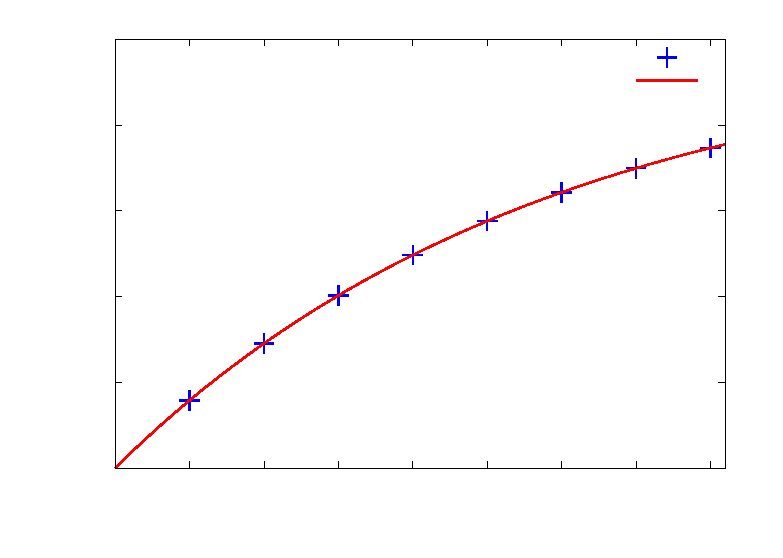
\includegraphics{plots/T1Polarisationsfeldfeld}}%
    \gplfronttext
  \end{picture}%
\endgroup

    \caption[T$_{1,p}$ measurement by varying $\tau_p$ and observing how the attenuation $\frac{\text{E}}{\text{E}_0}$ evolves.]{T$_{1,p}$ measurement by varying $\tau_p$ and observing how the attenuation $\frac{\text{E}}{\text{E}_0}$ evolves.
    The provided exponential fit results in a value for T$_{1,p}$ of \SI{2912.8800 \pm 0.0048}{\milli \second}.}
    \label{fig:T1Polarisationsfeldfeld}
\end{figure}

The second option is to calculate the spin lattice relaxation via the earths magnetic field B$_e$.
In this case the index will be chosen as "$e$" for the spin lattice relaxation.
The procedure in this case is to change the time $t$ (pre-90 minimum delay) between the polarizing pulse ends and the \SI{90}{\degree} pulse begins.
This relation is also visualized in figure \ref{fig:BildT1}.
The pre-90 minimum delay is chosen as \SI{0}{\milli \second} and the pre-90 delay step size as \SI{500}{\milli \second}.
For every configuration the signal maximum is calculated again of the fourier transformed spectrum.
Figure \ref{fig:T1Erdmagnetfeld} shows the attenuation of the signals normalized to the maximum peak E$_0$.
This time the T$_{1,e}$ can be calculated by the following fit function:
\begin{align}
    S(x) = S_0 \cdot \exp\left(\frac{-x}{T_{1,e}}\right) \ .
    \label{eq: fitBe}
\end{align}
In our case T$_{1,e}$ is observed to be \SI{2753.0500 \pm 0.0012}{\milli \second}.\newline
In both ways the uncertainty of the T$_1$ values are quite small.
This is the result of really good aligned values to the fit function.
Nevertheless T$_{1,p}$ and T$_{1,e}$ are not consistent even though the uncertainty is considered.
This might be, due to the fact that those two measurements are based on two different methods and T$_{1,e}$ is dependent on the earths magnetic field.
Even though they are not consistent, the values for T$_{1,p}$ and T$_{1,e}$ have the same magnitude and also have the same magnitude according to a literature value of \SI{4000}{\milli \second} \cite{literaturT1}.
It is good to keep in mind that a comparison to literature values is just there to get the magnitude.
Since the surrounding magnetic field and the probe define the exact value.
\begin{figure}[H]
    \centering
    % GNUPLOT: LaTeX picture with Postscript
\begingroup
  % Encoding inside the plot.  In the header of your document, this encoding
  % should to defined, e.g., by using
  % \usepackage[cp1252,<other encodings>]{inputenc}
  \inputencoding{cp1252}%
  \makeatletter
  \providecommand\color[2][]{%
    \GenericError{(gnuplot) \space\space\space\@spaces}{%
      Package color not loaded in conjunction with
      terminal option `colourtext'%
    }{See the gnuplot documentation for explanation.%
    }{Either use 'blacktext' in gnuplot or load the package
      color.sty in LaTeX.}%
    \renewcommand\color[2][]{}%
  }%
  \providecommand\includegraphics[2][]{%
    \GenericError{(gnuplot) \space\space\space\@spaces}{%
      Package graphicx or graphics not loaded%
    }{See the gnuplot documentation for explanation.%
    }{The gnuplot epslatex terminal needs graphicx.sty or graphics.sty.}%
    \renewcommand\includegraphics[2][]{}%
  }%
  \providecommand\rotatebox[2]{#2}%
  \@ifundefined{ifGPcolor}{%
    \newif\ifGPcolor
    \GPcolorfalse
  }{}%
  \@ifundefined{ifGPblacktext}{%
    \newif\ifGPblacktext
    \GPblacktexttrue
  }{}%
  % define a \g@addto@macro without @ in the name:
  \let\gplgaddtomacro\g@addto@macro
  % define empty templates for all commands taking text:
  \gdef\gplbacktext{}%
  \gdef\gplfronttext{}%
  \makeatother
  \ifGPblacktext
    % no textcolor at all
    \def\colorrgb#1{}%
    \def\colorgray#1{}%
  \else
    % gray or color?
    \ifGPcolor
      \def\colorrgb#1{\color[rgb]{#1}}%
      \def\colorgray#1{\color[gray]{#1}}%
      \expandafter\def\csname LTw\endcsname{\color{white}}%
      \expandafter\def\csname LTb\endcsname{\color{black}}%
      \expandafter\def\csname LTa\endcsname{\color{black}}%
      \expandafter\def\csname LT0\endcsname{\color[rgb]{1,0,0}}%
      \expandafter\def\csname LT1\endcsname{\color[rgb]{0,1,0}}%
      \expandafter\def\csname LT2\endcsname{\color[rgb]{0,0,1}}%
      \expandafter\def\csname LT3\endcsname{\color[rgb]{1,0,1}}%
      \expandafter\def\csname LT4\endcsname{\color[rgb]{0,1,1}}%
      \expandafter\def\csname LT5\endcsname{\color[rgb]{1,1,0}}%
      \expandafter\def\csname LT6\endcsname{\color[rgb]{0,0,0}}%
      \expandafter\def\csname LT7\endcsname{\color[rgb]{1,0.3,0}}%
      \expandafter\def\csname LT8\endcsname{\color[rgb]{0.5,0.5,0.5}}%
    \else
      % gray
      \def\colorrgb#1{\color{black}}%
      \def\colorgray#1{\color[gray]{#1}}%
      \expandafter\def\csname LTw\endcsname{\color{white}}%
      \expandafter\def\csname LTb\endcsname{\color{black}}%
      \expandafter\def\csname LTa\endcsname{\color{black}}%
      \expandafter\def\csname LT0\endcsname{\color{black}}%
      \expandafter\def\csname LT1\endcsname{\color{black}}%
      \expandafter\def\csname LT2\endcsname{\color{black}}%
      \expandafter\def\csname LT3\endcsname{\color{black}}%
      \expandafter\def\csname LT4\endcsname{\color{black}}%
      \expandafter\def\csname LT5\endcsname{\color{black}}%
      \expandafter\def\csname LT6\endcsname{\color{black}}%
      \expandafter\def\csname LT7\endcsname{\color{black}}%
      \expandafter\def\csname LT8\endcsname{\color{black}}%
    \fi
  \fi
    \setlength{\unitlength}{0.0500bp}%
    \ifx\gptboxheight\undefined%
      \newlength{\gptboxheight}%
      \newlength{\gptboxwidth}%
      \newsavebox{\gptboxtext}%
    \fi%
    \setlength{\fboxrule}{0.5pt}%
    \setlength{\fboxsep}{1pt}%
\begin{picture}(7200.00,5040.00)%
    \gplgaddtomacro\gplbacktext{%
      \csname LTb\endcsname%%
      \put(814,704){\makebox(0,0)[r]{\strut{}$0$}}%
      \put(814,1527){\makebox(0,0)[r]{\strut{}$0.2$}}%
      \put(814,2350){\makebox(0,0)[r]{\strut{}$0.4$}}%
      \put(814,3173){\makebox(0,0)[r]{\strut{}$0.6$}}%
      \put(814,3996){\makebox(0,0)[r]{\strut{}$0.8$}}%
      \put(814,4819){\makebox(0,0)[r]{\strut{}$1$}}%
      \put(946,484){\makebox(0,0){\strut{}$0$}}%
      \put(1660,484){\makebox(0,0){\strut{}$500$}}%
      \put(2375,484){\makebox(0,0){\strut{}$1000$}}%
      \put(3089,484){\makebox(0,0){\strut{}$1500$}}%
      \put(3803,484){\makebox(0,0){\strut{}$2000$}}%
      \put(4517,484){\makebox(0,0){\strut{}$2500$}}%
      \put(5232,484){\makebox(0,0){\strut{}$3000$}}%
      \put(5946,484){\makebox(0,0){\strut{}$3500$}}%
      \put(6660,484){\makebox(0,0){\strut{}$4000$}}%
    }%
    \gplgaddtomacro\gplfronttext{%
      \csname LTb\endcsname%%
      \put(209,2761){\rotatebox{-270}{\makebox(0,0){\strut{}Attenuation $\frac{\text{E}}{\text{E}_0}$}}}%
      \put(3874,154){\makebox(0,0){\strut{}Time between pulses $t$ in $\si{\milli \second}$}}%
      \csname LTb\endcsname%%
      \put(5816,4646){\makebox(0,0)[r]{\strut{}measured values}}%
      \csname LTb\endcsname%%
      \put(5816,4426){\makebox(0,0)[r]{\strut{}attenuation-Fit}}%
    }%
    \gplbacktext
    \put(0,0){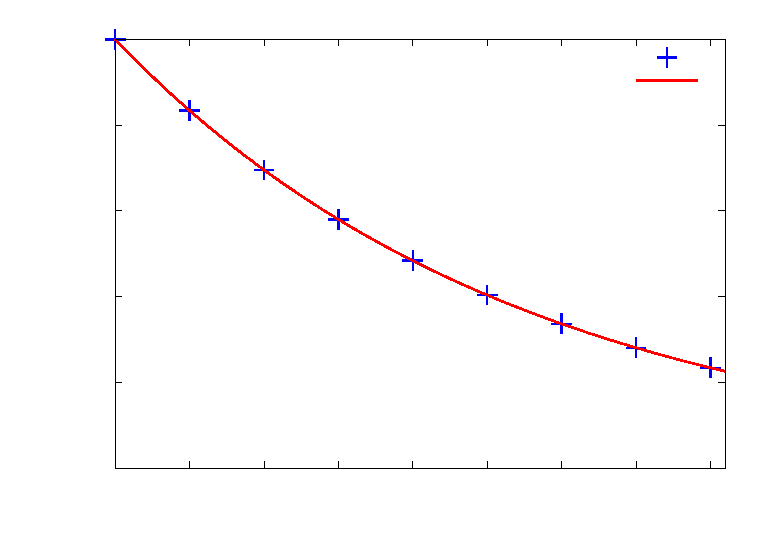
\includegraphics{plots/T1Erdmagnetfeld}}%
    \gplfronttext
  \end{picture}%
\endgroup

    \caption[T$_{1,e}$ measurement by varying $t$ and observing how the attenuation $\frac{\text{E}}{\text{E}_0}$ evolves.]{T$_{1,e}$ measurement by varying $t$ and observing how the attenuation $\frac{\text{E}}{\text{E}_0}$ evolves.
    The provided exponential fit results in a value for T$_{1,e}$ of \SI{2753.0500 \pm 0.0012}{\milli \second}.}
    \label{fig:T1Erdmagnetfeld}
\end{figure}